\documentclass[12pt, oneside]{article}

% Language setting
% Replace `english' with e.g. `spanish' to change the document language
\usepackage[english]{babel}

% Set page size and margins
% Replace `letterpaper' with `a4paper' for UK/EU standard size
\usepackage[letterpaper,top=2cm,bottom=2cm,left=3cm,right=3cm,marginparwidth=1.75cm]{geometry}

% Useful packages
\usepackage{amsmath}
\usepackage{graphicx}
\usepackage[colorlinks=true, allcolors=blue]{hyperref}
\usepackage{graphicx} % Required for inserting images
\usepackage{cite}
\usepackage{amsmath,amssymb,amsfonts}
\usepackage{algorithmic}
\usepackage{graphicx}
\usepackage{textcomp}
\usepackage{xcolor}
\usepackage{csquotes}
\usepackage{placeins}
\usepackage{etoolbox}
\usepackage{IEEEtrantools}

\begin{document}

\begin{titlepage}
    \begin{center}
        \vspace*{1cm}
        {\huges
        \center{\huge{\textbf{Advanced Control and Dynamics}}}}
         \\
         \vspace{0.3cm}
         \large{Coursework Report}
         \vspace{0.5cm}
        \\
        {\large By}
        \\
        \vspace{0.5cm}
        \textbf{Runze Yuan}
        \\
        \vspace{0.5cm}
        Student Number: 22071714
   		\vspace{1.5cm}
        \\
        \vspace{0.25cm}
       
\includegraphics[scale=0.6]{logos/bristolcrest_colour.pdf}
        \hspace{5mm}
        
\includegraphics[scale=0.35]{logos/UWE_insignia.png}

        \vspace{10mm}
        {\large Department of Engineering Mathematics\\
        \textsc{University of Bristol}}
        \\
        \&
        \\
        {\large Department of Engineering Design and Mathematics\\
        \textsc{University of the West of England}}\\

        \vspace{0.8cm}
 
        \vspace{0.8cm}
        \today
        
    \end{center}
    
\end{titlepage}

\tableofcontents
\pagebreak

\section{Practical Plant Definition}

% http://sim.okawa-denshi.jp/en/CRCRkeisan.htm


\textbf{Question:} 
\begin{quote}
Define a practical engineering plant which would feature similar dynamical behaviour to the theoretical dynamics given in the plant description below. Briefly describe the operation of the plant.
\end{quote}

Theoretical transfer function of the plant:

\begin{equation}
    \frac{Y(s)}{U(s)} = g_{p}(s) = \frac{1}{s^{2}+0.6s+4}
\end{equation}
\textbf{Answer:}
% https://electronics.stackexchange.com/questions/152159/deriving-2nd-order-passive-low-pass-filter-cutoff-frequency
\vspace{0.5cm}


\begin{figure}[htbp]
  \begin{minipage}[t]{0.5\textwidth}
    \centering
    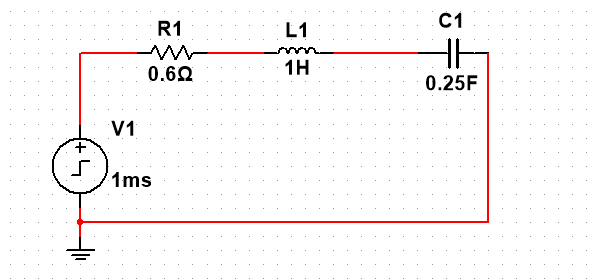
\includegraphics[width=\linewidth]{Report/pics/RLC电路例子.png}
    \caption{Example of RLC circuit. 
    \centering
    \begin{Large}
    $\frac{U_c}{V_1} = \frac{4}{s^2+0.6s+4}$.
    \end{Large}
    }
    \label{fig:RLC circuit example}
  \end{minipage}
  \hfill
  \begin{minipage}[t]{0.5\textwidth}
    \centering
    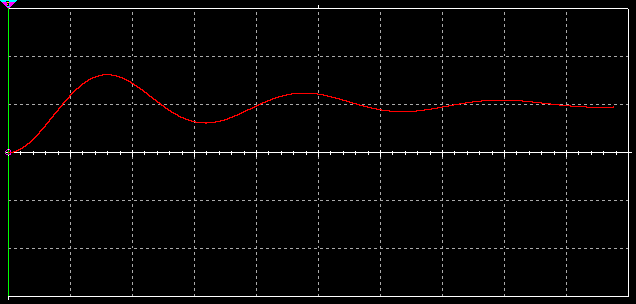
\includegraphics[width=\linewidth]{Report/pics/RLCStepResponse.png}
    \caption{Simulated step response of voltage across capacitor C1. }
    \label{fig:Uc step response}
  \end{minipage}
\end{figure}

A common example which has similar dynamic with the given transfer function is a RLC circuit.

As shown in Fig. \ref{fig:RLC circuit example}, the voltage across the capacitor C1 exhibits dynamic characteristics similar to the given transfer function. Explains are as follows:

\vspace{0.2cm}
Voltage equation of the entire circuit in time domain:
\begin{equation}
    V_1 = U_R+U_L+U_C = R\times I+L\times \frac{dI}{dt}+\frac{1}{C}\int_0^t Idt
    \label{equ:VoltageInTimeDomain}
\end{equation}

Apply Laplacian transform on equation (\ref{equ:VoltageInTimeDomain}), and we have:
\begin{equation}
        V_1(s) = RI(s)+ LI(s)s+\frac{I(s)}{Cs}
        \label{equ:VoltageInSDomain}
\end{equation}

And from equation (\ref{equ:VoltageInSDomain}), the relation of voltage across the capacitor and the source is:
\begin{equation}
    \frac{U_C(s)}{V_1(s)}=\frac{1}{LCs^2+CRs+1}
\end{equation}

Which have similar dynamic with the theoretical plant provided. The simulated step response of voltage across capacitor C1 is shown in Fig. \ref{fig:Uc step response}.

\pagebreak

\section{Control System Block Diagrams}
\textbf{Question:}
\begin{quote}
    Draw two equivalent control system block diagrams, which features the output feedback and the state feedback respectively. Compare the similarity and difference. 
\end{quote}
\textbf{Answer:}

\begin{figure}
    \centering
    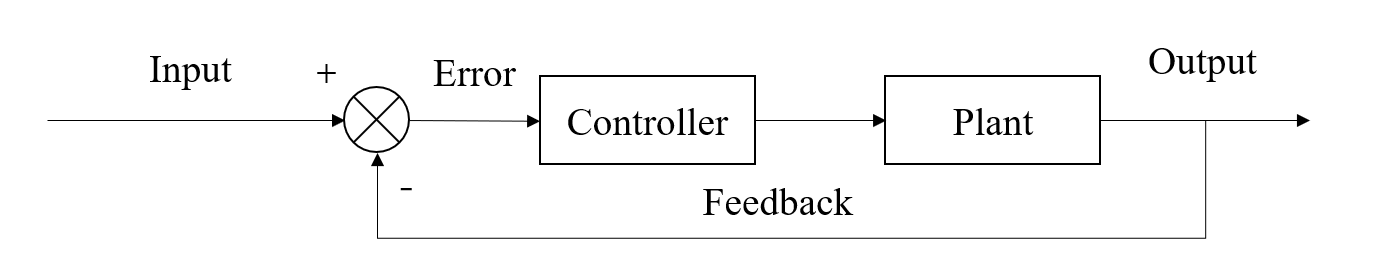
\includegraphics[width = \linewidth]{Report/pics/OutputFeedbackDiagram.png}
    \caption{Caption}
    \label{fig:my_label}
\end{figure}

\begin{figure}
    \centering
    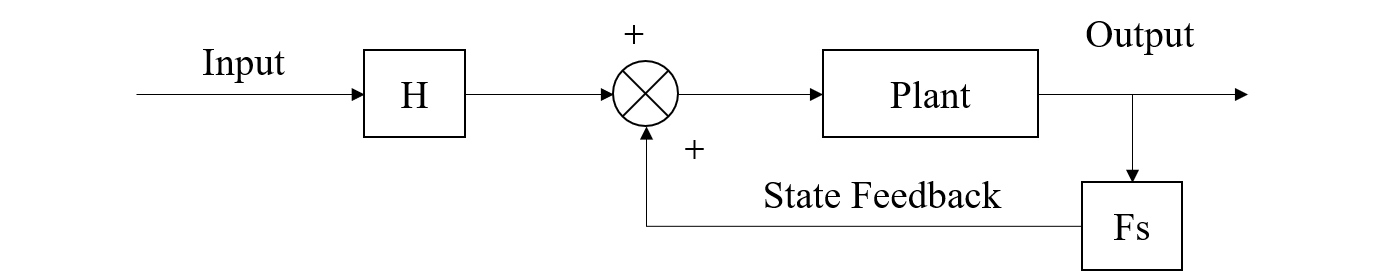
\includegraphics[width = \linewidth]{Report/pics/StateFeedbackDiagram.png}
    \caption{Caption}
    \label{fig:my_label}
\end{figure}


\section{Plant Analyse}
\section{State Feedback Controller Design}
\section{Observer Design}
\section{Performance Simulation}
\section{Digital Controller Implementation}
\section{References}

\end{document}